\chapter{Appendiks} \label{cha:AppD}
\textit{Dette appendiks indeholder forskellige instruktioner som Sygehusapoteket Region Nordjylland anvender i forbindelse med Amgrosskift. Det forekommer i følgende rækkefølge:}

\begin{enumerate}
\item Implementering af lægemiddelskift - skabelon til vurdering. 
\\Angivet i Appendiks på side \ref{XXX} og i litteraturlisten som~\citep{Sygehusapoteket2017}.  \label{item:ATC-ansvarlig}
%\item Amgrosudbud - Estimering af lægemiddelforbrug og opfølgning. Angivet i litteraturlisten som~\citep{Sygehusapoteket2017a}
%\item Implementering af lægemiddelskift. Angivet i litteraturlisten som~\citep{Sygehusapoteket2017b}
%\item Risikolægemidler lægemidler. \label{item:Risikolaegemidler} Angivet i litteraturlisten som [XX]
\item Skiftelister. Angivet i litteraturlisten som [XX] \label{item:Skiftelister}
\item Lægemiddel Nyt - Amgrosudbud og lægemiddelskift \label{item:Laegemiddelnyt}. Angivet i litteraturlisten som [XX] 
\end{enumerate}




%\includepdf[scale=0.8,pages=2-15,pagecommand={}]{mypages}
%\includepdf[scale=0.8,pages=16,pagecommand={}\label{appendix:bslut}]{mypages}
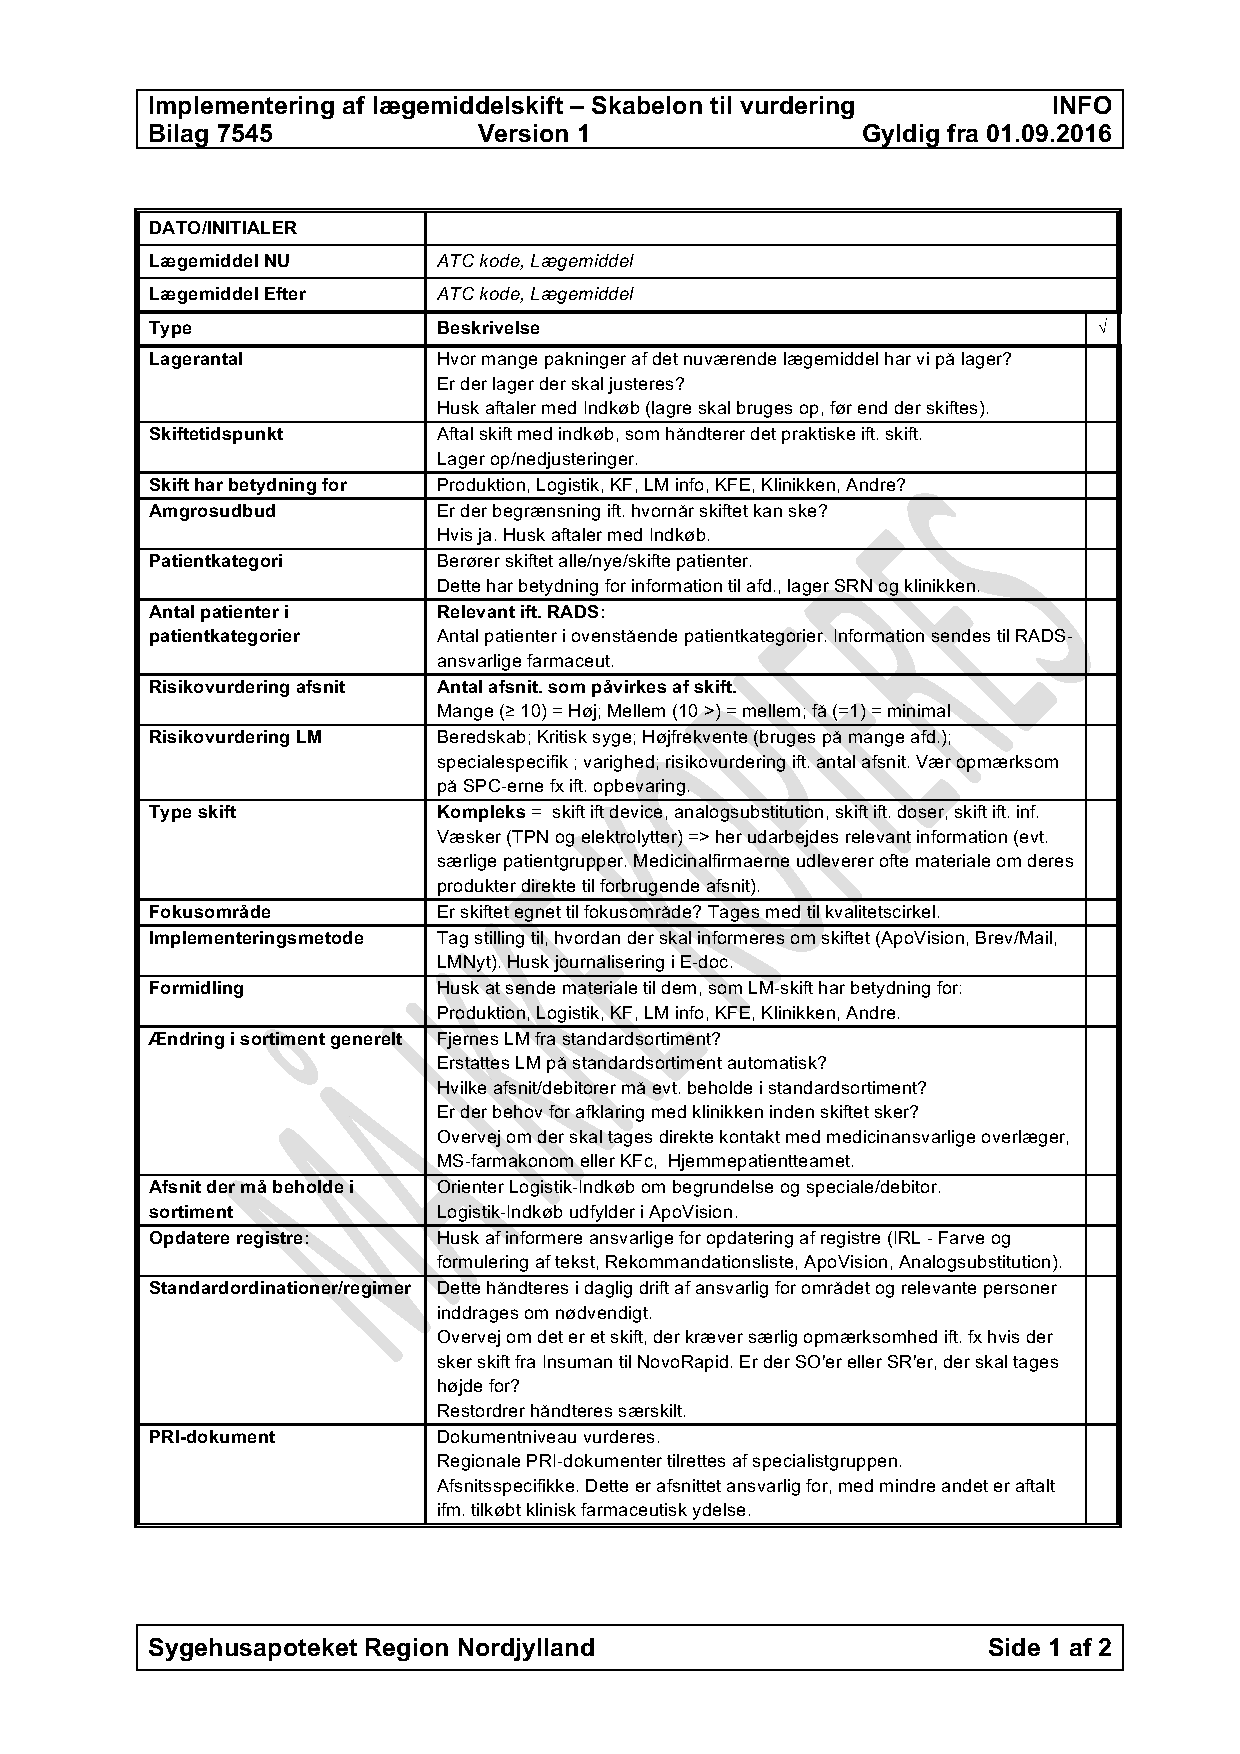
\includepdf[pages=1]{appendiks/Skabelon.pdf} 
%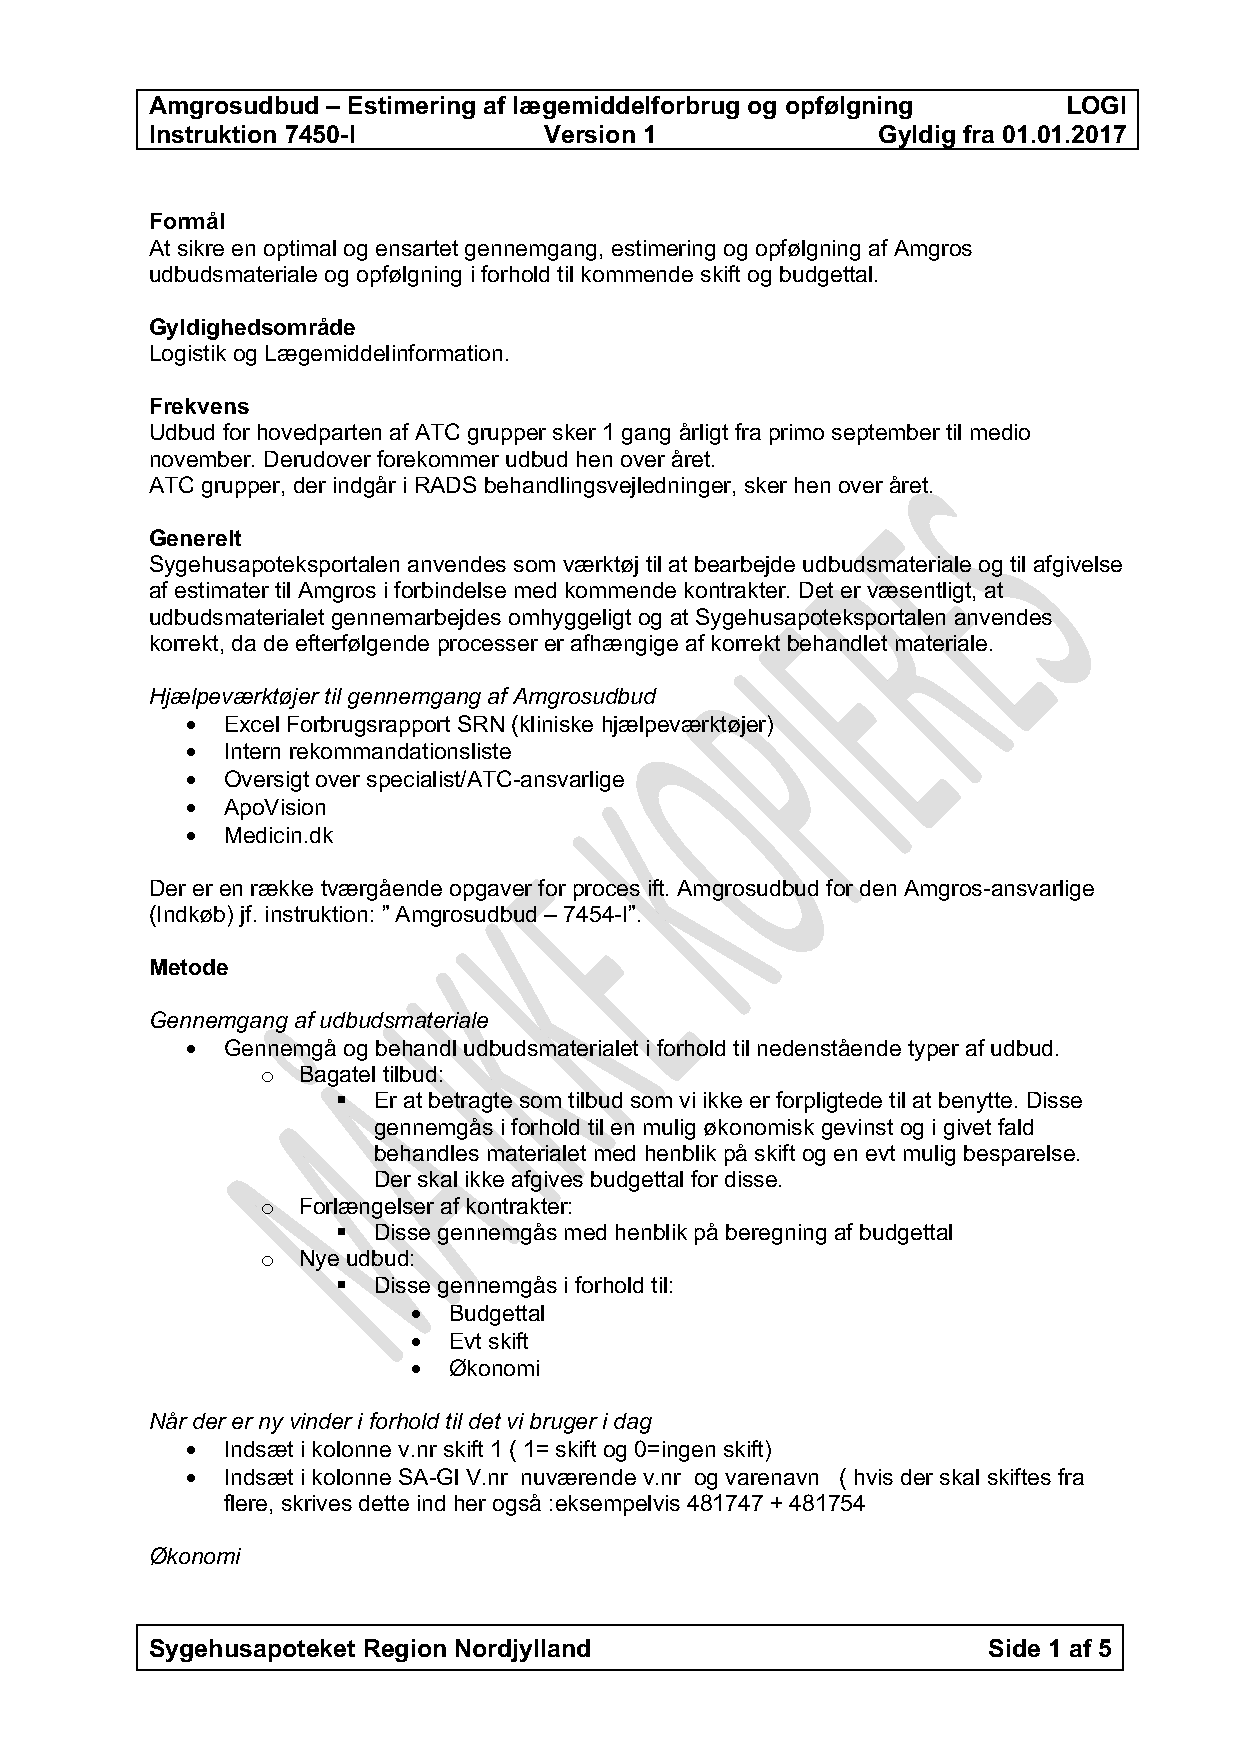
\includepdf[pages=1-3]{appendiks/Estimering.pdf}
%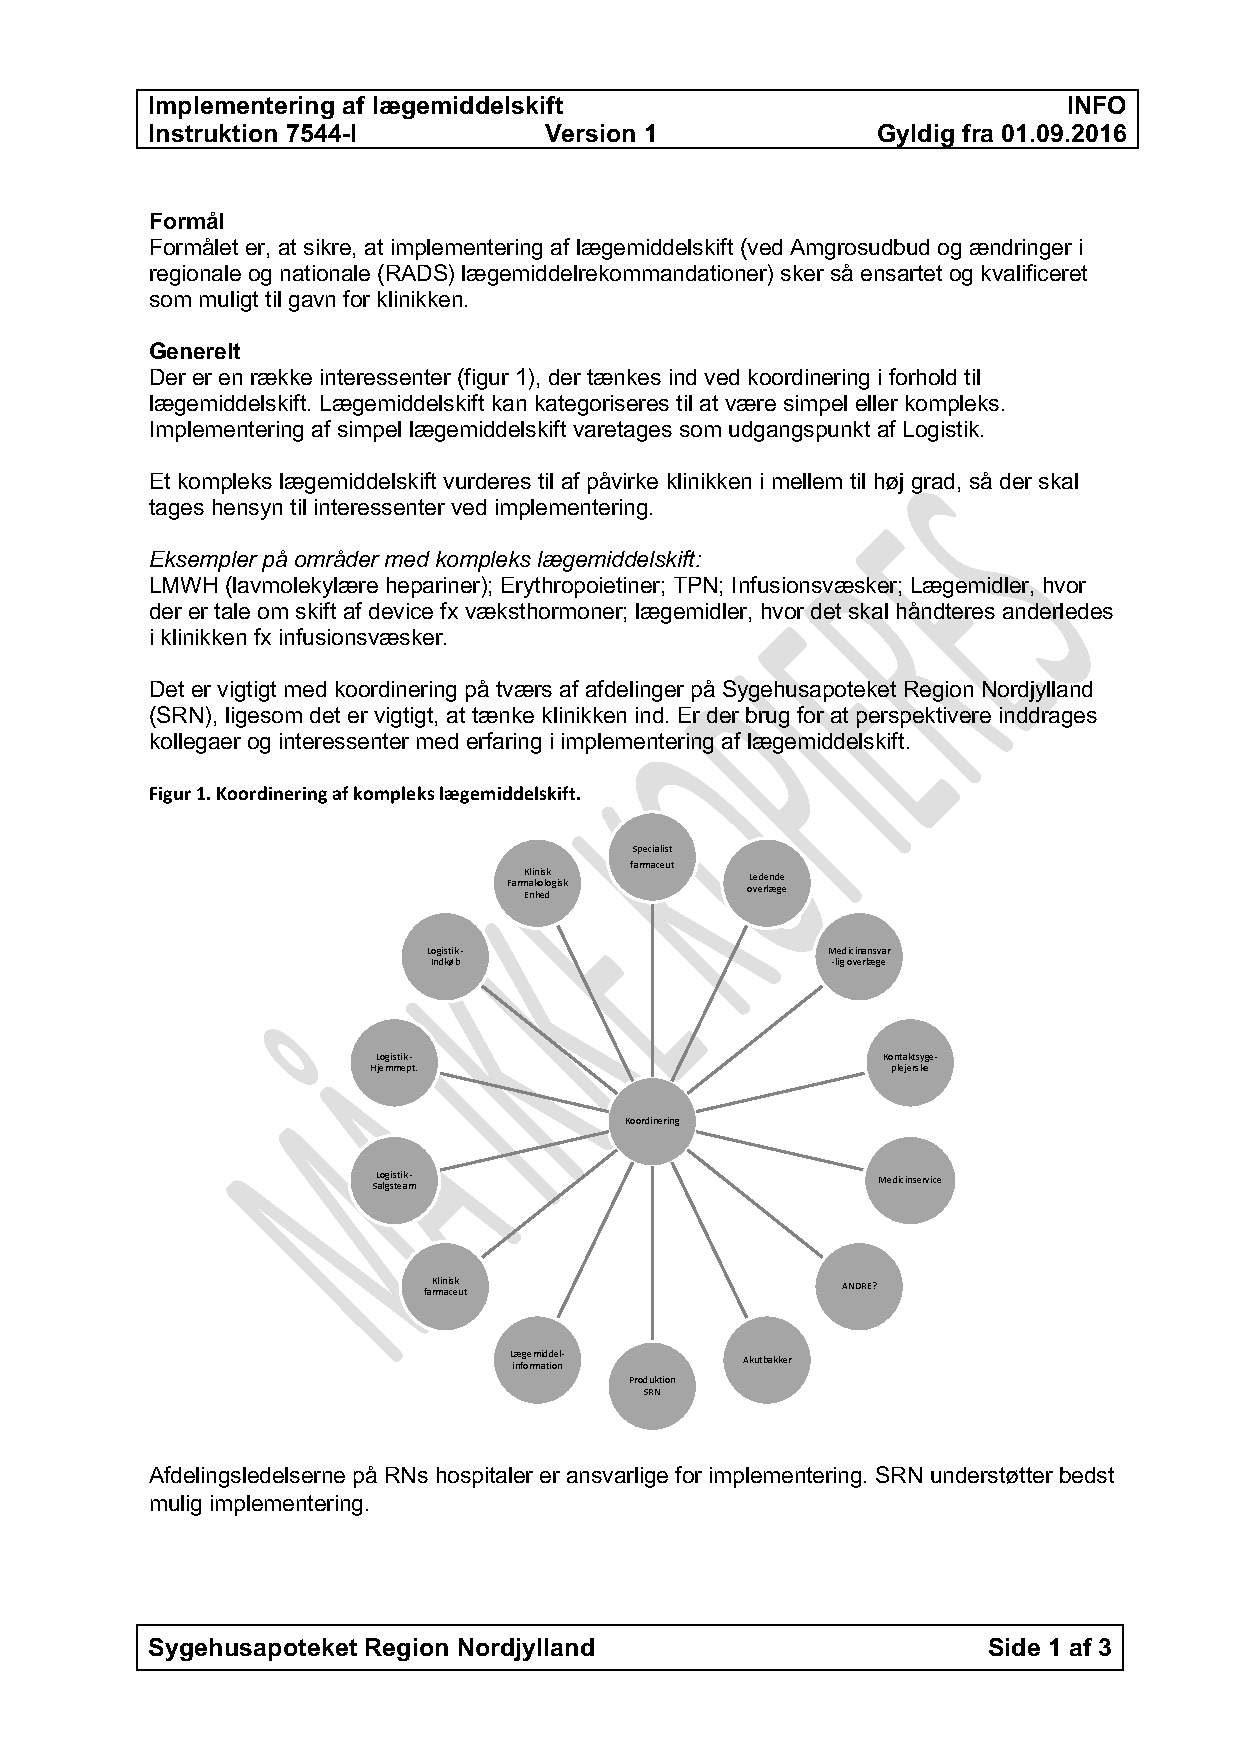
\includepdf[pages=1-2]{appendiks/Instruktion.pdf}
%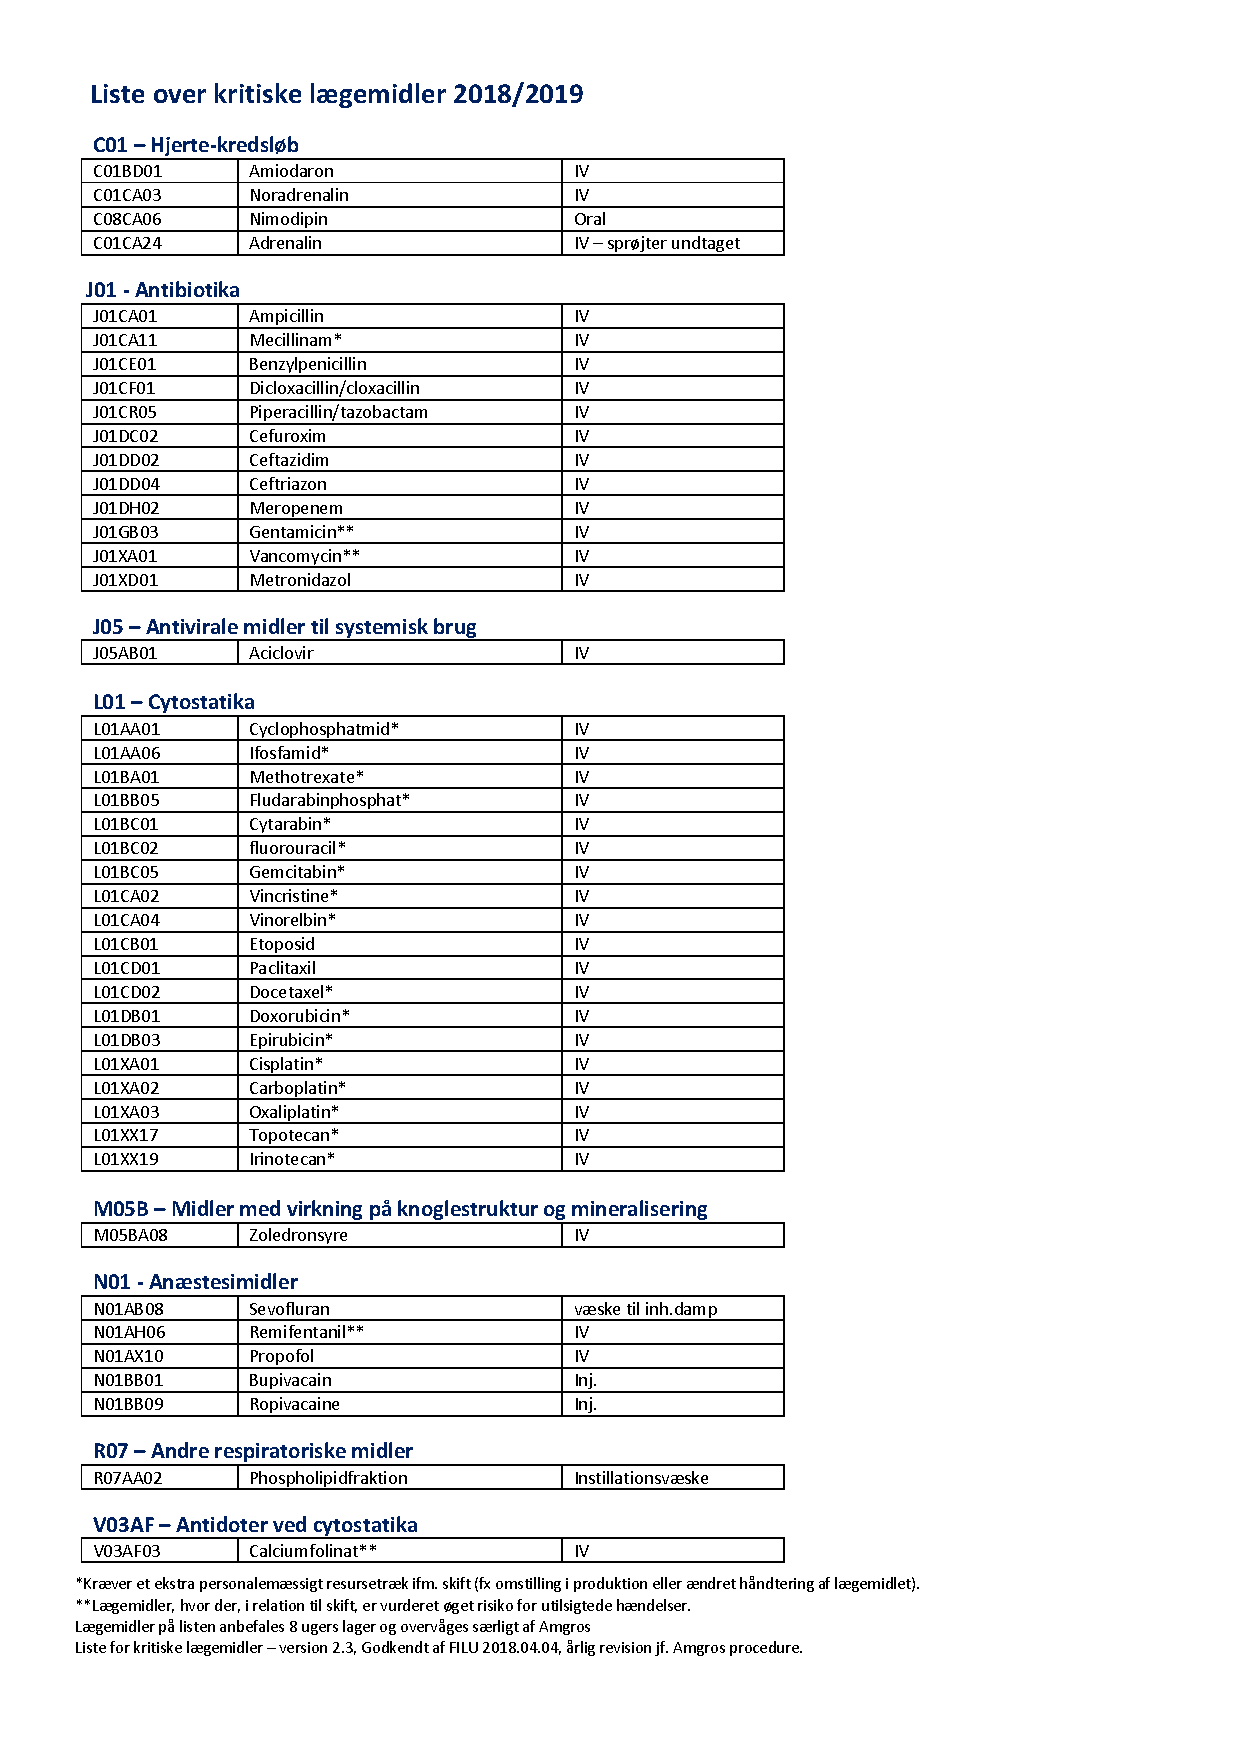
\includepdf[pages=1]{appendiks/Kistisklaegemidler.pdf}
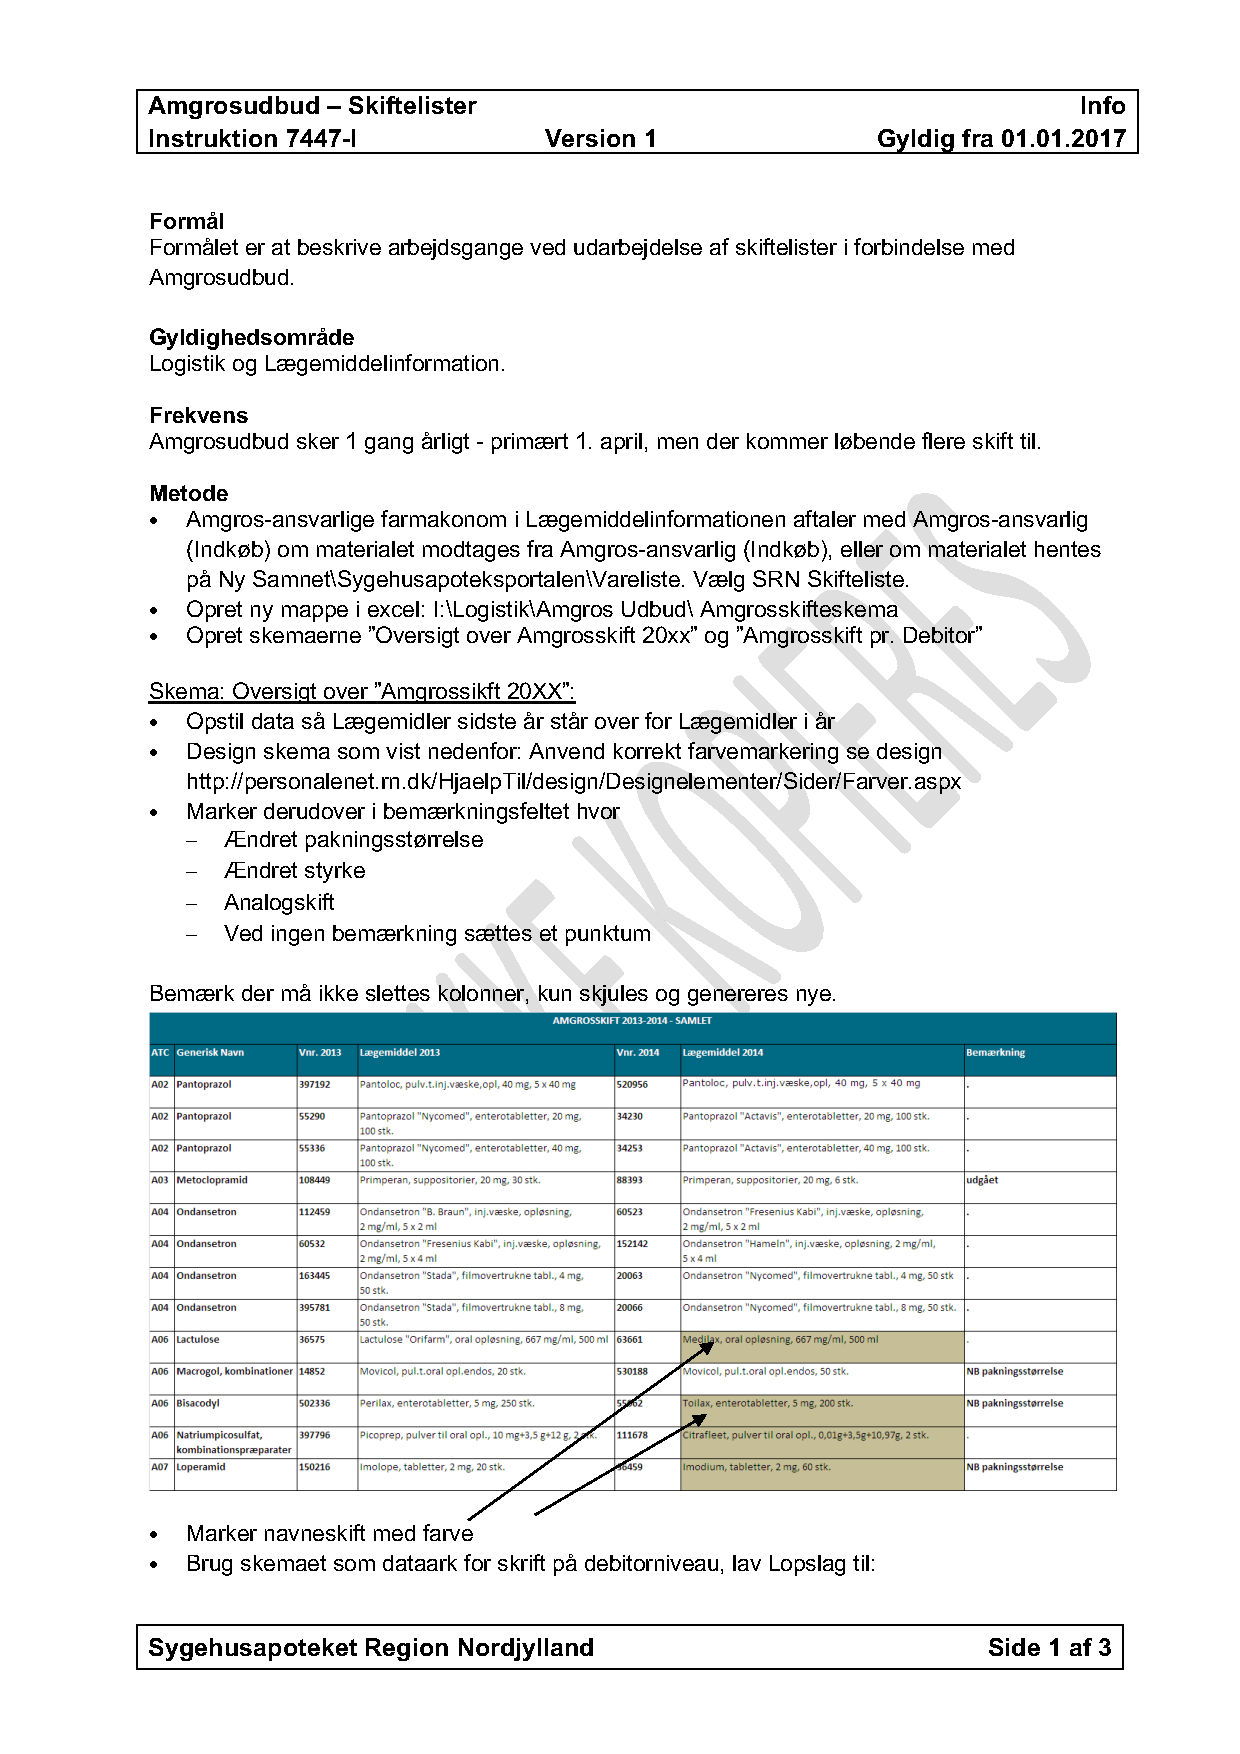
\includepdf[pages=1-3]{appendiks/Skiftelister.pdf}
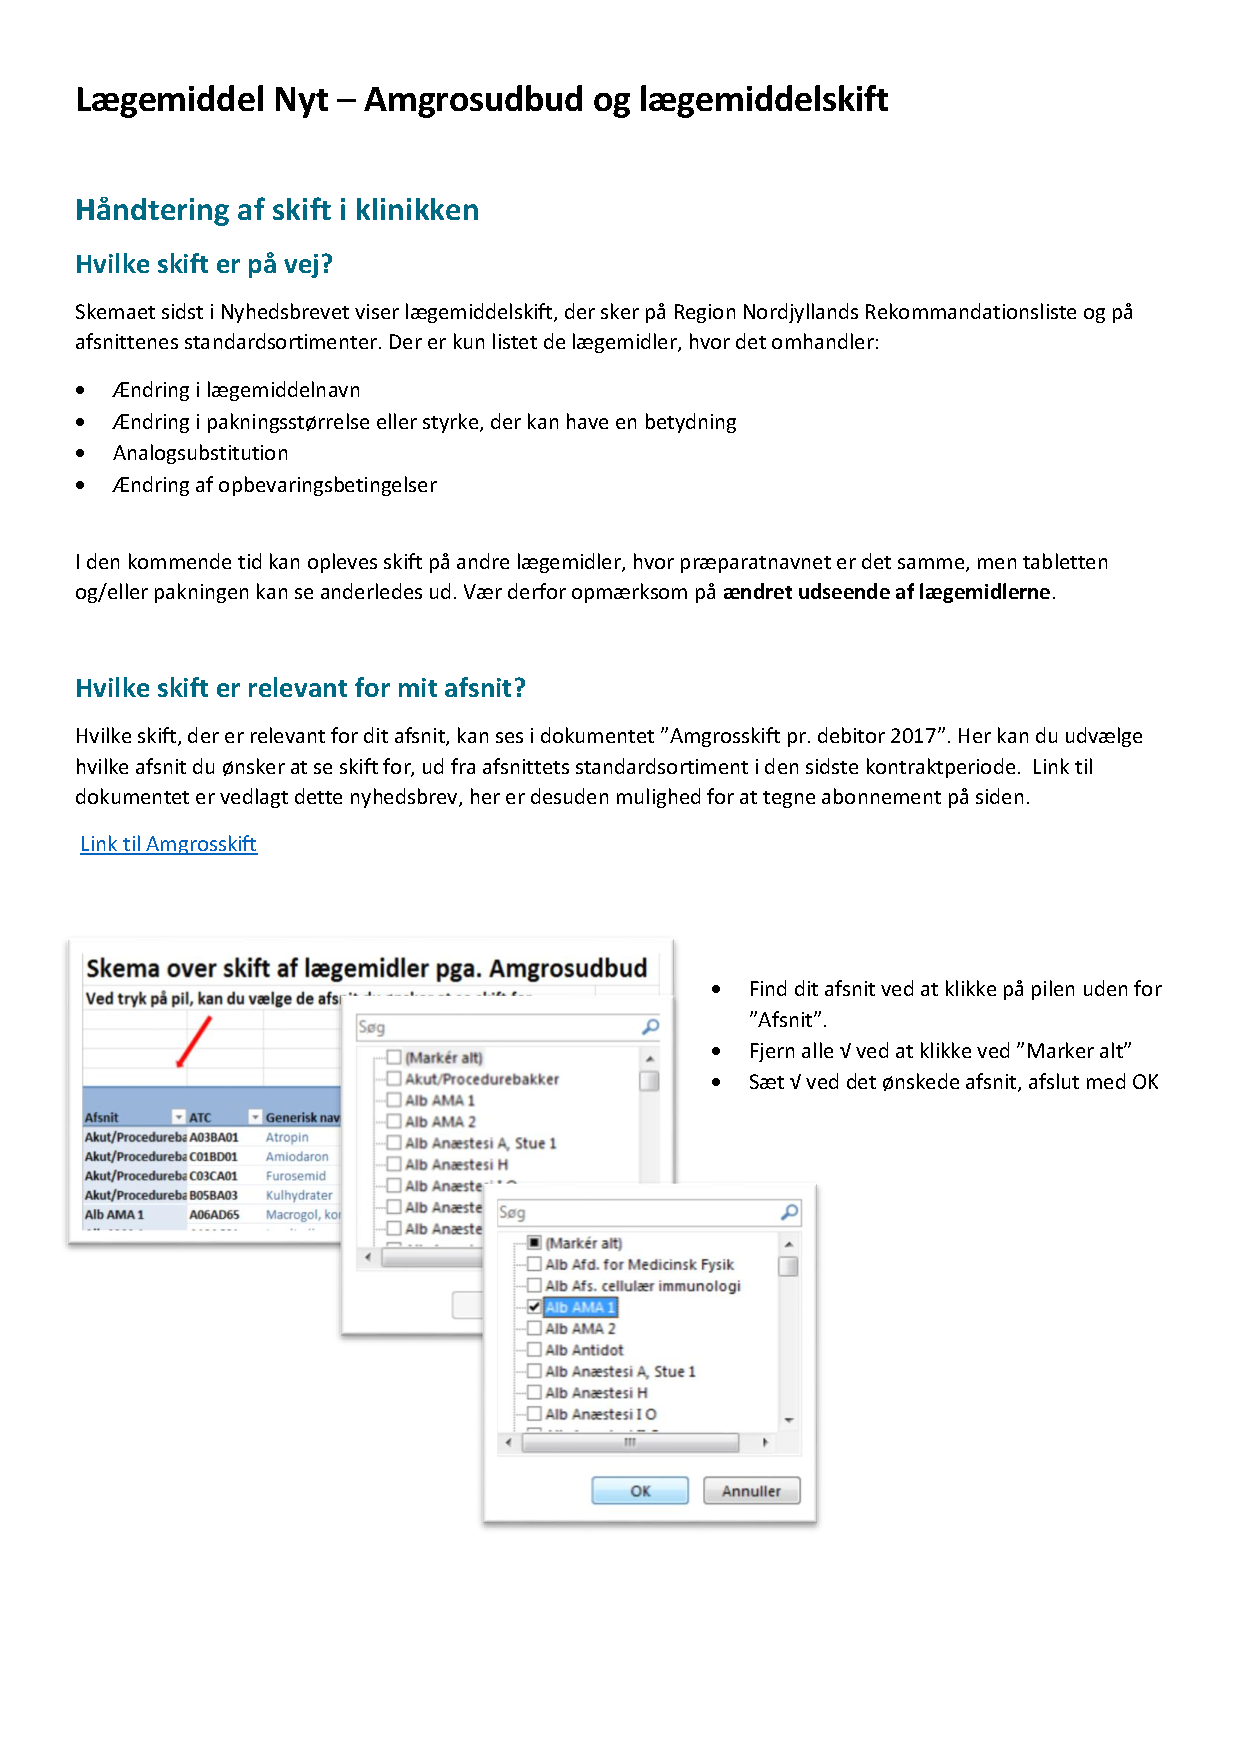
\includepdf[pages=1-10]{appendiks/Laegemiddelnyt.pdf}